\subsection{Pourquoi décomposer la table ?}
\paragraph{}{Il y a au début une unique table contenant une vingtaine d'attributs. Pour illustrer la redondance et les dépendances fonctionnelles, cet exemple de \textit{tuples} ne sera centré que sur quelques attributs pour des raisons de lisibilité. La figure \ref{bigtableex} présente un aperçu de notre \textit{big table}.}

\begin{figure}
    {
	\centering
    \begin{tabular}{|l|l|l|l|l|l|l|l|}
        \hline idArt & titreArt & idJrnal & typeJrnal & idCont & nomCont & nomPers & nomMetier \\ 
        \hline 1 & Les pieuvres & 1 & Hebdo & 1 & Photo & Bertrand & Photographe \\ 
        \hline 1 & Les pieuvres & 1 & Hebdo & 2 &Texte & Nadine & Redacteur \\ 
        \hline 2 & Manger du sel & 1 & Hebdo & 3 & Schéma & Yves & Infographie \\ 
        \hline 2 & Manger du sel & 1 & Hebdo & 4 & Texte & Nadine & Redacteur \\ 
        \hline 3 & Critique film & 1 & Hebdo & 5 & Texte & Manon & Critique \\ 
        \hline 4 & Des poissons & 3 & HS & 6 & Texte & Nadine & Redacteur \\ 
        \hline 2 & Manger du sel & 3 & HS & 1 & Schéma & Yves & Infographie \\ 
        \hline 2 & Manger du sel & 3 & HS & 2 & Texte & Nadine & Redacteur \\ 
        \hline 
    \end{tabular}
    \label{bigtableex}
    }
\caption{Exemple de \textit{tuples} dans la \textit{big table} (vue partielle)}
\end{figure} 

\paragraph{}{On remarque qu'il a une répétition des données relatives au journal ou au contenu : un contenu a toujours les mêmes ID, nom et auteur associé. Les journaux d'un même ID ont leur type en commun, de même pour les identifiants des articles et leurs titres. Enfin, les personnes ont toujours le même métier. On peut avoir une perte d'information du fait de cette configuration car si l'on supprime par exemple tous les contenus créés par une personne, on perd les données qui lui sont associées, à savoir son nom, son prénom, son numéro, etc.}

\paragraph{}{De ce fait, en prenant en compte tous les attributs nous avons dégagé un ensemble de dépendances fonctionnelles.}

\begin{figure}
	\centering
	\ifx\du\undefined
  \newlength{\du}
\fi
\setlength{\du}{15\unitlength}
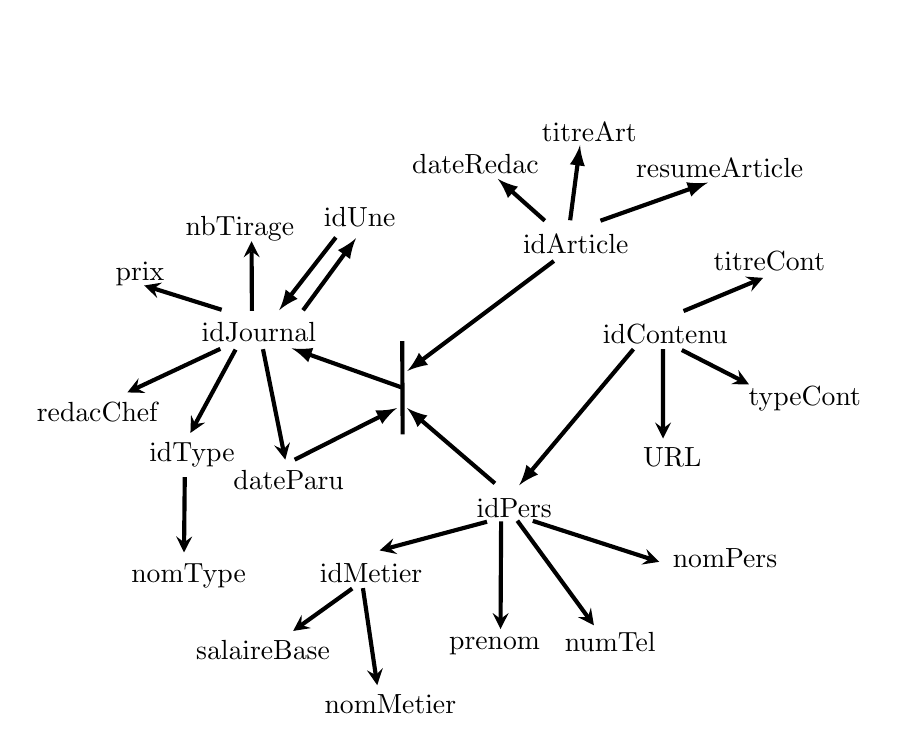
\begin{tikzpicture}[scale=0.9]
\pgftransformxscale{1.000000}
\pgftransformyscale{-1.000000}
\definecolor{dialinecolor}{rgb}{0.000000, 0.000000, 0.000000}
\pgfsetstrokecolor{dialinecolor}
\definecolor{dialinecolor}{rgb}{1.000000, 1.000000, 1.000000}
\pgfsetfillcolor{dialinecolor}
% setfont left to latex
\definecolor{dialinecolor}{rgb}{0.000000, 0.000000, 0.000000}
\pgfsetstrokecolor{dialinecolor}
\node[anchor=west] at (29.900000\du,17.850000\du){idPers};
% setfont left to latex
\definecolor{dialinecolor}{rgb}{0.000000, 0.000000, 0.000000}
\pgfsetstrokecolor{dialinecolor}
\node[anchor=west] at (35.150000\du,19.200000\du){nomPers};
% setfont left to latex
\definecolor{dialinecolor}{rgb}{0.000000, 0.000000, 0.000000}
\pgfsetstrokecolor{dialinecolor}
\node[anchor=west] at (29.163689\du,21.565612\du){prenom};
% setfont left to latex
\definecolor{dialinecolor}{rgb}{0.000000, 0.000000, 0.000000}
\pgfsetstrokecolor{dialinecolor}
\node[anchor=west] at (32.259087\du,21.436290\du){numTel};
% setfont left to latex
\definecolor{dialinecolor}{rgb}{0.000000, 0.000000, 0.000000}
\pgfsetstrokecolor{dialinecolor}
\node[anchor=west] at (25.706125\du,19.600000\du){idMetier};
% setfont left to latex
\definecolor{dialinecolor}{rgb}{0.000000, 0.000000, 0.000000}
\pgfsetstrokecolor{dialinecolor}
\node[anchor=west] at (30.500000\du,21.600000\du){};
% setfont left to latex
\definecolor{dialinecolor}{rgb}{0.000000, 0.000000, 0.000000}
\pgfsetstrokecolor{dialinecolor}
\node[anchor=west] at (25.828978\du,23.102844\du){nomMetier};
\pgfsetlinewidth{0.100000\du}
\pgfsetdash{}{0pt}
\pgfsetdash{}{0pt}
\pgfsetbuttcap
{
\definecolor{dialinecolor}{rgb}{0.000000, 0.000000, 0.000000}
\pgfsetfillcolor{dialinecolor}
% was here!!!
\pgfsetarrowsend{stealth}
\definecolor{dialinecolor}{rgb}{0.000000, 0.000000, 0.000000}
\pgfsetstrokecolor{dialinecolor}
\draw (30.437875\du,18.227601\du)--(27.564463\du,18.995588\du);
}
\pgfsetlinewidth{0.100000\du}
\pgfsetdash{}{0pt}
\pgfsetdash{}{0pt}
\pgfsetbuttcap
{
\definecolor{dialinecolor}{rgb}{0.000000, 0.000000, 0.000000}
\pgfsetfillcolor{dialinecolor}
% was here!!!
\pgfsetarrowsend{stealth}
\definecolor{dialinecolor}{rgb}{0.000000, 0.000000, 0.000000}
\pgfsetstrokecolor{dialinecolor}
\draw (30.816138\du,18.216138\du)--(30.800000\du,21.100000\du);
}
\pgfsetlinewidth{0.100000\du}
\pgfsetdash{}{0pt}
\pgfsetdash{}{0pt}
\pgfsetbuttcap
{
\definecolor{dialinecolor}{rgb}{0.000000, 0.000000, 0.000000}
\pgfsetfillcolor{dialinecolor}
% was here!!!
\pgfsetarrowsend{stealth}
\definecolor{dialinecolor}{rgb}{0.000000, 0.000000, 0.000000}
\pgfsetstrokecolor{dialinecolor}
\draw (31.250000\du,18.200000\du)--(33.300000\du,21.000000\du);
}
\pgfsetlinewidth{0.100000\du}
\pgfsetdash{}{0pt}
\pgfsetdash{}{0pt}
\pgfsetbuttcap
{
\definecolor{dialinecolor}{rgb}{0.000000, 0.000000, 0.000000}
\pgfsetfillcolor{dialinecolor}
% was here!!!
\pgfsetarrowsend{stealth}
\definecolor{dialinecolor}{rgb}{0.000000, 0.000000, 0.000000}
\pgfsetstrokecolor{dialinecolor}
\draw (31.664363\du,18.204676\du)--(35.050000\du,19.300000\du);
}
\pgfsetlinewidth{0.100000\du}
\pgfsetdash{}{0pt}
\pgfsetdash{}{0pt}
\pgfsetbuttcap
{
\definecolor{dialinecolor}{rgb}{0.000000, 0.000000, 0.000000}
\pgfsetfillcolor{dialinecolor}
% was here!!!
\pgfsetarrowsend{stealth}
\definecolor{dialinecolor}{rgb}{0.000000, 0.000000, 0.000000}
\pgfsetstrokecolor{dialinecolor}
\draw (27.117425\du,20.004288\du)--(27.500000\du,22.600000\du);
}
% setfont left to latex
\definecolor{dialinecolor}{rgb}{0.000000, 0.000000, 0.000000}
\pgfsetstrokecolor{dialinecolor}
\node[anchor=west] at (22.500000\du,13.150000\du){idJournal};
% setfont left to latex
\definecolor{dialinecolor}{rgb}{0.000000, 0.000000, 0.000000}
\pgfsetstrokecolor{dialinecolor}
\node[anchor=west] at (18.088100\du,15.300000\du){redacChef};
% setfont left to latex
\definecolor{dialinecolor}{rgb}{0.000000, 0.000000, 0.000000}
\pgfsetstrokecolor{dialinecolor}
\node[anchor=west] at (23.348812\du,17.097434\du){dateParu};
% setfont left to latex
\definecolor{dialinecolor}{rgb}{0.000000, 0.000000, 0.000000}
\pgfsetstrokecolor{dialinecolor}
\node[anchor=west] at (21.096837\du,16.438537\du){idType};
% setfont left to latex
\definecolor{dialinecolor}{rgb}{0.000000, 0.000000, 0.000000}
\pgfsetstrokecolor{dialinecolor}
\node[anchor=west] at (20.198549\du,11.592687\du){prix};
% setfont left to latex
\definecolor{dialinecolor}{rgb}{0.000000, 0.000000, 0.000000}
\pgfsetstrokecolor{dialinecolor}
\node[anchor=west] at (22.069695\du,10.376113\du){nbTirage};
\pgfsetlinewidth{0.100000\du}
\pgfsetdash{}{0pt}
\pgfsetdash{}{0pt}
\pgfsetbuttcap
{
\definecolor{dialinecolor}{rgb}{0.000000, 0.000000, 0.000000}
\pgfsetfillcolor{dialinecolor}
% was here!!!
\pgfsetarrowsend{stealth}
\definecolor{dialinecolor}{rgb}{0.000000, 0.000000, 0.000000}
\pgfsetstrokecolor{dialinecolor}
\draw (23.300000\du,13.600000\du)--(20.812463\du,14.765925\du);
}
\pgfsetlinewidth{0.100000\du}
\pgfsetdash{}{0pt}
\pgfsetdash{}{0pt}
\pgfsetbuttcap
{
\definecolor{dialinecolor}{rgb}{0.000000, 0.000000, 0.000000}
\pgfsetfillcolor{dialinecolor}
% was here!!!
\pgfsetarrowsend{stealth}
\definecolor{dialinecolor}{rgb}{0.000000, 0.000000, 0.000000}
\pgfsetstrokecolor{dialinecolor}
\draw (23.708460\du,13.619674\du)--(22.500000\du,15.850000\du);
}
\pgfsetlinewidth{0.100000\du}
\pgfsetdash{}{0pt}
\pgfsetdash{}{0pt}
\pgfsetbuttcap
{
\definecolor{dialinecolor}{rgb}{0.000000, 0.000000, 0.000000}
\pgfsetfillcolor{dialinecolor}
% was here!!!
\pgfsetarrowsend{stealth}
\definecolor{dialinecolor}{rgb}{0.000000, 0.000000, 0.000000}
\pgfsetstrokecolor{dialinecolor}
\draw (24.442061\du,13.608212\du)--(25.038323\du,16.565538\du);
}
\pgfsetlinewidth{0.100000\du}
\pgfsetdash{}{0pt}
\pgfsetdash{}{0pt}
\pgfsetbuttcap
{
\definecolor{dialinecolor}{rgb}{0.000000, 0.000000, 0.000000}
\pgfsetfillcolor{dialinecolor}
% was here!!!
\pgfsetarrowsend{stealth}
\definecolor{dialinecolor}{rgb}{0.000000, 0.000000, 0.000000}
\pgfsetstrokecolor{dialinecolor}
\draw (22.348439\du,17.035500\du)--(22.327700\du,19.050000\du);
}
\pgfsetlinewidth{0.100000\du}
\pgfsetdash{}{0pt}
\pgfsetdash{}{0pt}
\pgfsetbuttcap
{
\definecolor{dialinecolor}{rgb}{0.000000, 0.000000, 0.000000}
\pgfsetfillcolor{dialinecolor}
% was here!!!
\pgfsetarrowsend{stealth}
\definecolor{dialinecolor}{rgb}{0.000000, 0.000000, 0.000000}
\pgfsetstrokecolor{dialinecolor}
\draw (23.335575\du,12.554150\du)--(21.263275\du,11.904150\du);
}
\pgfsetlinewidth{0.100000\du}
\pgfsetdash{}{0pt}
\pgfsetdash{}{0pt}
\pgfsetbuttcap
{
\definecolor{dialinecolor}{rgb}{0.000000, 0.000000, 0.000000}
\pgfsetfillcolor{dialinecolor}
% was here!!!
\pgfsetarrowsend{stealth}
\definecolor{dialinecolor}{rgb}{0.000000, 0.000000, 0.000000}
\pgfsetstrokecolor{dialinecolor}
\draw (24.145850\du,12.581225\du)--(24.135338\du,10.719661\du);
}
% setfont left to latex
\definecolor{dialinecolor}{rgb}{0.000000, 0.000000, 0.000000}
\pgfsetstrokecolor{dialinecolor}
\node[anchor=west] at (31.100000\du,10.800000\du){idArticle};
% setfont left to latex
\definecolor{dialinecolor}{rgb}{0.000000, 0.000000, 0.000000}
\pgfsetstrokecolor{dialinecolor}
\node[anchor=west] at (28.400000\du,5.250000\du){};
% setfont left to latex
\definecolor{dialinecolor}{rgb}{0.000000, 0.000000, 0.000000}
\pgfsetstrokecolor{dialinecolor}
\node[anchor=west] at (31.605687\du,7.800000\du){titreArt};
% setfont left to latex
\definecolor{dialinecolor}{rgb}{0.000000, 0.000000, 0.000000}
\pgfsetstrokecolor{dialinecolor}
\node[anchor=west] at (28.131821\du,8.650000\du){dateRedac};
% setfont left to latex
\definecolor{dialinecolor}{rgb}{0.000000, 0.000000, 0.000000}
\pgfsetstrokecolor{dialinecolor}
\node[anchor=west] at (33.239777\du,13.200000\du){idContenu};
% setfont left to latex
\definecolor{dialinecolor}{rgb}{0.000000, 0.000000, 0.000000}
\pgfsetstrokecolor{dialinecolor}
\node[anchor=west] at (36.200000\du,11.250000\du){titreCont};
% setfont left to latex
\definecolor{dialinecolor}{rgb}{0.000000, 0.000000, 0.000000}
\pgfsetstrokecolor{dialinecolor}
\node[anchor=west] at (34.313643\du,16.500000\du){URL};
% setfont left to latex
\definecolor{dialinecolor}{rgb}{0.000000, 0.000000, 0.000000}
\pgfsetstrokecolor{dialinecolor}
\node[anchor=west] at (37.139777\du,14.936933\du){typeCont};
\pgfsetlinewidth{0.100000\du}
\pgfsetdash{}{0pt}
\pgfsetdash{}{0pt}
\pgfsetbuttcap
{
\definecolor{dialinecolor}{rgb}{0.000000, 0.000000, 0.000000}
\pgfsetfillcolor{dialinecolor}
% was here!!!
\pgfsetarrowsend{stealth}
\definecolor{dialinecolor}{rgb}{0.000000, 0.000000, 0.000000}
\pgfsetstrokecolor{dialinecolor}
\draw (35.699164\du,12.588049\du)--(37.827700\du,11.700000\du);
}
\pgfsetlinewidth{0.100000\du}
\pgfsetdash{}{0pt}
\pgfsetdash{}{0pt}
\pgfsetbuttcap
{
\definecolor{dialinecolor}{rgb}{0.000000, 0.000000, 0.000000}
\pgfsetfillcolor{dialinecolor}
% was here!!!
\pgfsetarrowsend{stealth}
\definecolor{dialinecolor}{rgb}{0.000000, 0.000000, 0.000000}
\pgfsetstrokecolor{dialinecolor}
\draw (35.148964\du,13.608212\du)--(35.150000\du,16.000000\du);
}
\pgfsetlinewidth{0.100000\du}
\pgfsetdash{}{0pt}
\pgfsetdash{}{0pt}
\pgfsetbuttcap
{
\definecolor{dialinecolor}{rgb}{0.000000, 0.000000, 0.000000}
\pgfsetfillcolor{dialinecolor}
% was here!!!
\pgfsetarrowsend{stealth}
\definecolor{dialinecolor}{rgb}{0.000000, 0.000000, 0.000000}
\pgfsetstrokecolor{dialinecolor}
\draw (35.653314\du,13.631137\du)--(37.450000\du,14.550000\du);
}
% setfont left to latex
\definecolor{dialinecolor}{rgb}{0.000000, 0.000000, 0.000000}
\pgfsetstrokecolor{dialinecolor}
\node[anchor=west] at (22.350000\du,21.665911\du){salaireBase};
\pgfsetlinewidth{0.100000\du}
\pgfsetdash{}{0pt}
\pgfsetdash{}{0pt}
\pgfsetbuttcap
{
\definecolor{dialinecolor}{rgb}{0.000000, 0.000000, 0.000000}
\pgfsetfillcolor{dialinecolor}
% was here!!!
\pgfsetarrowsend{stealth}
\definecolor{dialinecolor}{rgb}{0.000000, 0.000000, 0.000000}
\pgfsetstrokecolor{dialinecolor}
\draw (26.830862\du,20.015751\du)--(25.250000\du,21.150000\du);
}
\pgfsetlinewidth{0.100000\du}
\pgfsetdash{}{0pt}
\pgfsetdash{}{0pt}
\pgfsetbuttcap
{
\definecolor{dialinecolor}{rgb}{0.000000, 0.000000, 0.000000}
\pgfsetfillcolor{dialinecolor}
% was here!!!
\pgfsetarrowsend{latex}
\definecolor{dialinecolor}{rgb}{0.000000, 0.000000, 0.000000}
\pgfsetstrokecolor{dialinecolor}
\draw (34.358051\du,13.608212\du)--(31.300000\du,17.250000\du);
}
\pgfsetlinewidth{0.100000\du}
\pgfsetdash{}{0pt}
\pgfsetdash{}{0pt}
\pgfsetbuttcap
{
\definecolor{dialinecolor}{rgb}{0.000000, 0.000000, 0.000000}
\pgfsetfillcolor{dialinecolor}
% was here!!!
\pgfsetarrowsend{latex}
\definecolor{dialinecolor}{rgb}{0.000000, 0.000000, 0.000000}
\pgfsetstrokecolor{dialinecolor}
\draw (30.650000\du,17.200000\du)--(28.298990\du,15.185069\du);
}
\pgfsetlinewidth{0.100000\du}
\pgfsetdash{}{0pt}
\pgfsetdash{}{0pt}
\pgfsetbuttcap
{
\definecolor{dialinecolor}{rgb}{0.000000, 0.000000, 0.000000}
\pgfsetfillcolor{dialinecolor}
% was here!!!
\pgfsetarrowsend{latex}
\definecolor{dialinecolor}{rgb}{0.000000, 0.000000, 0.000000}
\pgfsetstrokecolor{dialinecolor}
\draw (32.227700\du,11.250000\du)--(28.304924\du,14.192800\du);
}
\pgfsetlinewidth{0.100000\du}
\pgfsetdash{}{0pt}
\pgfsetdash{}{0pt}
\pgfsetbuttcap
{
\definecolor{dialinecolor}{rgb}{0.000000, 0.000000, 0.000000}
\pgfsetfillcolor{dialinecolor}
% was here!!!
\definecolor{dialinecolor}{rgb}{0.000000, 0.000000, 0.000000}
\pgfsetstrokecolor{dialinecolor}
\draw (28.169049\du,13.390424\du)--(28.180511\du,15.889250\du);
}
% setfont left to latex
\definecolor{dialinecolor}{rgb}{0.000000, 0.000000, 0.000000}
\pgfsetstrokecolor{dialinecolor}
\node[anchor=west] at (20.614633\du,19.665911\du){nomType};
\pgfsetlinewidth{0.100000\du}
\pgfsetdash{}{0pt}
\pgfsetdash{}{0pt}
\pgfsetbuttcap
{
\definecolor{dialinecolor}{rgb}{0.000000, 0.000000, 0.000000}
\pgfsetfillcolor{dialinecolor}
% was here!!!
\pgfsetarrowsend{latex}
\definecolor{dialinecolor}{rgb}{0.000000, 0.000000, 0.000000}
\pgfsetstrokecolor{dialinecolor}
\draw (25.290499\du,16.565538\du)--(28.025700\du,15.185069\du);
}
\pgfsetlinewidth{0.100000\du}
\pgfsetdash{}{0pt}
\pgfsetdash{}{0pt}
\pgfsetbuttcap
{
\definecolor{dialinecolor}{rgb}{0.000000, 0.000000, 0.000000}
\pgfsetfillcolor{dialinecolor}
% was here!!!
\pgfsetarrowsend{latex}
\definecolor{dialinecolor}{rgb}{0.000000, 0.000000, 0.000000}
\pgfsetstrokecolor{dialinecolor}
\draw (28.174780\du,14.639837\du)--(25.210048\du,13.585287\du);
}
% setfont left to latex
\definecolor{dialinecolor}{rgb}{0.000000, 0.000000, 0.000000}
\pgfsetstrokecolor{dialinecolor}
\node[anchor=west] at (34.127700\du,8.750000\du){resumeArticle};
\pgfsetlinewidth{0.100000\du}
\pgfsetdash{}{0pt}
\pgfsetdash{}{0pt}
\pgfsetbuttcap
{
\definecolor{dialinecolor}{rgb}{0.000000, 0.000000, 0.000000}
\pgfsetfillcolor{dialinecolor}
% was here!!!
\pgfsetarrowsend{latex}
\definecolor{dialinecolor}{rgb}{0.000000, 0.000000, 0.000000}
\pgfsetstrokecolor{dialinecolor}
\draw (31.985313\du,10.169461\du)--(30.727700\du,9.050000\du);
}
\pgfsetlinewidth{0.100000\du}
\pgfsetdash{}{0pt}
\pgfsetdash{}{0pt}
\pgfsetbuttcap
{
\definecolor{dialinecolor}{rgb}{0.000000, 0.000000, 0.000000}
\pgfsetfillcolor{dialinecolor}
% was here!!!
\pgfsetarrowsend{latex}
\definecolor{dialinecolor}{rgb}{0.000000, 0.000000, 0.000000}
\pgfsetstrokecolor{dialinecolor}
\draw (32.663911\du,10.157999\du)--(32.927700\du,8.150000\du);
}
\pgfsetlinewidth{0.100000\du}
\pgfsetdash{}{0pt}
\pgfsetdash{}{0pt}
\pgfsetbuttcap
{
\definecolor{dialinecolor}{rgb}{0.000000, 0.000000, 0.000000}
\pgfsetfillcolor{dialinecolor}
% was here!!!
\pgfsetarrowsend{latex}
\definecolor{dialinecolor}{rgb}{0.000000, 0.000000, 0.000000}
\pgfsetstrokecolor{dialinecolor}
\draw (33.475438\du,10.169461\du)--(36.350000\du,9.150000\du);
}
\pgfsetlinewidth{0.100000\du}
\pgfsetdash{}{0pt}
\pgfsetdash{}{0pt}
\pgfsetbuttcap
{
\definecolor{dialinecolor}{rgb}{0.000000, 0.000000, 0.000000}
\pgfsetfillcolor{dialinecolor}
% was here!!!
\pgfsetarrowsend{latex}
\definecolor{dialinecolor}{rgb}{0.000000, 0.000000, 0.000000}
\pgfsetstrokecolor{dialinecolor}
\draw (26.392361\du,10.616499\du)--(24.875525\du,12.564625\du);
}
% setfont left to latex
\definecolor{dialinecolor}{rgb}{0.000000, 0.000000, 0.000000}
\pgfsetstrokecolor{dialinecolor}
\node[anchor=west] at (25.772362\du,10.080562\du){idUne};
\pgfsetlinewidth{0.100000\du}
\pgfsetdash{}{0pt}
\pgfsetdash{}{0pt}
\pgfsetbuttcap
{
\definecolor{dialinecolor}{rgb}{0.000000, 0.000000, 0.000000}
\pgfsetfillcolor{dialinecolor}
% was here!!!
\pgfsetarrowsend{latex}
\definecolor{dialinecolor}{rgb}{0.000000, 0.000000, 0.000000}
\pgfsetstrokecolor{dialinecolor}
\draw (25.514962\du,12.567137\du)--(26.931099\du,10.639424\du);
}
% setfont left to latex
\definecolor{dialinecolor}{rgb}{0.000000, 0.000000, 0.000000}
\pgfsetstrokecolor{dialinecolor}
\node[anchor=west] at (29.750000\du,21.450000\du){};
\end{tikzpicture}
	\caption{Schéma des dépendances fonctionnelles de la base de données}
	\label{sch_df}
\end{figure} 

\paragraph{Dépendances fonctionnelles}{Les dépendances fonctionnelles de la figure \ref{sch_df} peuvent être retranscrites de la manière suivante.
}
\begin{enumerate}
    \item[(1)] idJournal $\rightarrow$ prix, nbTirage, idUne, idType, redacChef, dateParu
    \item[(2)] idType $\rightarrow$ nomType
    \item[(3)] idUne $\rightarrow$ idJournal
    \item[(4)] idArticle $\rightarrow$ dateRedac, titreArt, resumeArt
    \item[(5)] idContenu $\rightarrow$ URL, titreCont, typeCont
    \item[(6)] idPers $\rightarrow$ nomPers, prenom, numTel, idMetier
    \item[(7)] idMetier $\rightarrow$ salaireBase, nomMetier
    \item[(8)] idArticle, idPers, dateParu $\rightarrow$ idJournal
\end{enumerate}

\paragraph{Clés}{
    De ce schéma, on peut en déduire trois clés $\{idJournal, idArticle, idContenu\}$, $\{idUne, idArticle, idContenu\}$ et $\{dateParu, idContenu, idArticle\}$. Ces ensembles d'attributs sont des clés, car ils déterminent l'ensemble des attributs.
}

\subsection{Algorithme de Bernstein}
\paragraph{}{Une fois nos dépendances fonctionnelles établies, nous commençons par appliquer l'algorithme de Bernstein pour décomposer notre grande table. Tout d'abord, nous déterminons sa couverture minimale. Pour cela, on utilise la clé \{idJournal, idArticle, idContenu\}.
}

\paragraph{}{
    Les dépendances (1), (4), (5), (6) et (7) ne sont pas élémentaires, nous avons donc dû les décomposer. Toutes les relations n'ont qu'un seul attributs à gauche, il n'est donc pas nécessaire de calculer la fermeture de ces attributs. Mais il est cependant nécessaire de le faire pour la dépendance (8) qui a plus d'un attribut en partie gauche.
    }

\paragraph{}{
    Calcul de la fermeture des attributs en partie gauche de la dépendance fonctionnelle (8) :
}
\begin{itemize}
    \item $idArticle+ = \{dateRedac, titreArt, resumeArticle\}$
    \item $idPers+ = \{nomPers, numTel, prenom, idMetier, nomMetier, salaireBase\}$
    \item $dateParu+ = \{\}$
\end{itemize}

\paragraph{}{Comme aucun élément des trois fermetures n'apparaît en partie gauche de la dépendance (8), cette dernière n'a pas besoin d'être modifiée.}
\paragraph{Couverture minimale}{
\begin{enumerate}
    \item[(1.1)] idJournal $\rightarrow$ prix
    \item[(1.2)] idJournal $\rightarrow$ nbTirage
    \item[(1.3)] idJournal $\rightarrow$ idUne
    \item[(1.4)] idJournal $\rightarrow$ idType
    \item[(1.5)] idJournal $\rightarrow$ redacChef
    \item[(1.6)] idJournal $\rightarrow$ dateParu
    \item[(2)] idType $\rightarrow$ nomType
    \item[(3)] idUne $\rightarrow$ idJournal
    \item[(4.1)] idArticle $\rightarrow$ dateRedac
    \item[(4.2)] idArticle $\rightarrow$ titreArt
    \item[(4.3)] idArticle $\rightarrow$ resumeArt
    \item[(5.1)] idContenu $\rightarrow$ URL
    \item[(5.2)] idContenu $\rightarrow$ titreCont
    \item[(5.3)] idContenu $\rightarrow$ typeCont
    \item[(6.1)] idPers $\rightarrow$ nomPers
    \item[(6.2)] idPers $\rightarrow$ prénom
    \item[(6.3)] idPers $\rightarrow$ numTel
    \item[(6.4)] idPers $\rightarrow$ idMetier
    \item[(7.1)] idMetier $\rightarrow$ salaireBase
    \item[(7.2)] idMetier $\rightarrow$ nomMetier
    \item[(8)] idArticle, idPers, dateParu $\rightarrow$ idJournal
\end{enumerate}}

\paragraph{}{
    Nous regroupons maintenant les dépendances ayant même partie gauche comme ci-dessous.
}
\begin{enumerate}
    \item[(1)] $DF_{1} = \{ (1.1), (1.2), (1.3), (1.4), (1.5), (1.6) \}$
    \item[(2)] $DF_{2} = \{ (2) \}$
    \item[(3)] $DF_{3} = \{ (3) \}$
    \item[(4)] $DF_{4} = \{ (4.1), (4.2), (4.3) \}$
    \item[(5)] $DF_{5} = \{ (5.1), (5.2), (5.3) \}$
    \item[(6)] $DF_{6} = \{ (6.1), (6.2), (6.3), (6.4) \}$
    \item[(7)] $DF_{7} = \{ (7.1), (7.2) \}$
    \item[(8)] $DF_{8} = \{ (8) \}$
\end{enumerate}

\paragraph{}{
    On construit à présent les schémas $<R_{i}(U_{i}), DF_{i}>$ pour chaque $DF_{i}$, où $U_{i}$ est l'ensemble des attributs apparaissant dans $DF_{i}$.
}
\begin{enumerate}
    \item[(1)] $<R_{1}(idJournal, nbTirage, idUne, idType, redacChef, dateParu), DF_{1}>$
    \item[(2)] $<R_{2}(idType, nomType),DF_{2}>$
    \item[(3)] $<R_{3}(idUne, idJournal),DF_{3}>$
    \item[(4)] $<R_{4}(idArticle, dateRedac, titreArt, resumeArt),DF_{4}>$
    \item[(5)] $<R_{5}(idContenu, URL, titreCont, typeCont),DF_{5}>$
    \item[(6)] $<R_{6}(idPers, nomPers, prenom, numTel, idMetier),DF_{6}>$
    \item[(7)] $<R_{7}(idMetier, salaireBase, nomMetier),DF_{7}>$
    \item[(8)] $<R_{8}(idArticle, idPers, dateParu, idJournal),DF_{8}>$
\end{enumerate}

\paragraph{}{
    Pour terminer, comme la clé entière n'étant pas présente dans le schéma, on l'ajoute le schéma suivant $<R_{9}(idJournal, idArticle, idContenu), \{\}>$.
}

\paragraph{}{
    Après avoir appliqué de l'algorithme de Bernstein sur notre table de départ, nous obtenons neuf relations. Ce schéma est sans perte d'informations, car la dernière relation permet de relier toutes les tables entre elles grâce à la clé, sans perte de dépendances fonctionnelles, car nous n'avons perdu aucune dépendance fonctionnelle par rapport au modèle de base et est en troisième forme normale, car l'algorithme nous le garantit.
}

\paragraph{}{
    Mais qu'en est-il pour l'algorithme de décomposition ? Donne-t il le même résultat?
}

\subsection{Algorithme de décomposition}
\paragraph{}{
    On considère la relation de départ \\
$R (idJournal, idContenu, idArticle, titreCont, typeCont, URL, dateRedac, \\
titreArt, resumeArticle, idPers, nomPers, numTel, prenom, idMetier,\\ 
salaireBase, nomMetier, dateParu, idUne, nbTirage, prix, \\
redacChef,  idType, nomType)$ avec les dépendances fonctionnelles énumérées au début de ce rapport, 
$DF = \{(1),(2),(3), ... ,(8)\}$.
}

\paragraph{}{
    On décompose la relation avec l'algorithme de décomposition vu en cours. Plusieurs résultats sont possibles. Dans cette exécution nous avons arbitrairement choisi l'ordre nous permettant de conserver les sous-ensembles les plus proches de la réalité de notre table. Les tables obtenues sont celles-ci :
}    
    
\begin{enumerate}
    \item[(Étape 1)] $R_1(idMetier, salaireBase, nomMetier), DF_1=\{(7)\}\\
    R_2(idJournal, idContenu, idArticle, titreCont, typeCont, URL, \\
    dateRedac, titreArt, resumeArticle, idPers, nomPers, numTel, \\
    prenom, idMetier, dateParu, idUne, nbTirage, prix, redacChef,\\
    idType, nomType), DF_2 = \{(1),(2),(3),(4),(5),(6),(8)\}$
    
    \item[(Étape 2)] $R_{21}(idType, nomType), DF_{21}=\{(2)\}\\
    R_{22}(idJournal, idContenu, idArticle, titreCont, typeCont, \\
    URL, dateRedac, titreArt, resumeArticle, idPers, nomPers, \\
    numTel, prenom, idMetier, dateParu, idUne, nbTirage, \\
    prix, redacChef,  idType), DF_{22} = \{(1),(3),(4),(5),(6),(8)\}$
    
    \item[(Étape 3)] $R_{221}(idPers, nomPers, prenom, numTel, idMetier), DF_{221}=\{(6)\}\\
    R_{222}(idJournal, idContenu, idArticle, titreCont, typeCont, URL,\\
    dateRedac, titreArt, resumeArticle, idPers, dateParu, idUne, \\
    nbTirage, prix, redacChef,  idType), DF_{222} = \{(1),(3),(4),(5),(8)\}$
    
    \item[(Étape 4)] $R_{2221}(idContenu, URL, idPers, titreCont, typeCont), DF_{2221}=\{(5)\}\\
    R_{2222}(idJournal, idContenu, idArticle, dateRedac, titreArt, \\
    resumeArticle, dateParu, idUne, nbTirage, prix, redacChef,  idType), \\
    DF_{2222} = \{(1),(3),(4),(8)\}$
    
    \item[(Étape 5)] $R_{22221}(idJournal, idUne, nbTirage, prix, redacChef, idType, dateParu),\\
    DF_{22221}=\{(1)\} \\
    R_{22222}(idJournal, idContenu, idArticle, dateRedac, titreArt, \\
    resumeArticle), DF_{22222} = \{(3),(4),(8)\}$
    
    \item[(Étape 6)] $R_{222221}(idArticle, dateRedac, titreArt, resumeArticle), DF_{222221}=\{(4)\}$ \\
    $R_{222222}(idArticle, idContenu, idJournal), DF_{222222}=\{()\}$
\end{enumerate}

\paragraph{}{On récupère ensuite les feuilles de l'arbre pour obtenir les tables à créer : $R_{2}, R_{22}, R_{222}, R_{2222}, R_{22222}, R_{222221} et R_{222222}$}

\paragraph{Choix du schéma}{
    Nous venons de voir deux décompositions différentes de notre table de départ. Il faut à présent choisir l'une des deux pour l'exploitation de nos données dans un système de gestion de base de données.
    
    Nous choisissons le résultat de l'algorithme de décomposition car le résultat est sans perte d'information et en troisième forme normale. Il s'approche en outre plus de la réalité de la façon dont on souhaite représenter les informations.
    
    Nous avons néanmoins remarqué que cette décomposition posait problème au niveau de la dernière table regroupant les attributs clé : dans notre cas, un numéro est composé d'articles lui-même composé de contenus. Dans le cas ou un article se retrouvait dans plus d'un numéro, on aurait eu une répétition de la composition des articles dans cette table, nous avons donc préféré la diviser en deux : d'une part une table d'association $(idArticle, idContenu)$ et d'autre part une autre table $(idJournal, idArticle)$. 
    
    On obtient donc le schéma de base de données représenté sur la figure \ref{schema_db}. Le fait de devoir effectuer cet ajustement indique peut-être une erreur dans la façon dont nous avons relevé nos dépendances fonctionnelles, une mauvaise exécution de l'algorithme de composition, ou une forme normale de niveau insuffisant.
    
}

\begin{figure}
    \centering
    %% Graphic for TeX using PGF
% Title: /comptes/E124582Q/L3/BDD/proj/wookie-hebdo/rapport/src/figures/tables_schema.dia
% Creator: Dia v0.97.2
% CreationDate: Fri Mar 20 13:48:47 2015
% For: E124582Q
% \usepackage{tikz}
% The following commands are not supported in PSTricks at present
% We define them conditionally, so when they are implemented,
% this pgf file will use them.
\ifx\du\undefined
  \newlength{\du}
\fi
\setlength{\du}{15\unitlength}
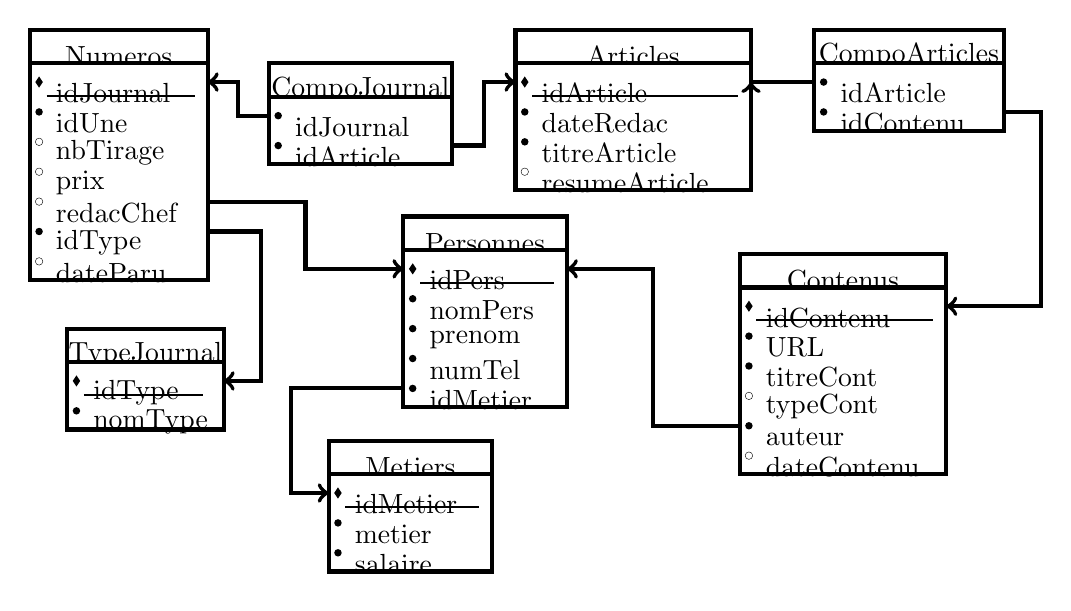
\begin{tikzpicture}[scale=0.9]
\pgftransformxscale{1.000000}
\pgftransformyscale{-1.000000}
\definecolor{dialinecolor}{rgb}{0.000000, 0.000000, 0.000000}
\pgfsetstrokecolor{dialinecolor}
\definecolor{dialinecolor}{rgb}{1.000000, 1.000000, 1.000000}
\pgfsetfillcolor{dialinecolor}
\pgfsetlinewidth{0.100000\du}
\pgfsetdash{}{0pt}
\definecolor{dialinecolor}{rgb}{1.000000, 1.000000, 1.000000}
\pgfsetfillcolor{dialinecolor}
\fill (12.000000\du,14.000000\du)--(12.000000\du,14.900000\du)--(16.380000\du,14.900000\du)--(16.380000\du,14.000000\du)--cycle;
\definecolor{dialinecolor}{rgb}{0.000000, 0.000000, 0.000000}
\pgfsetstrokecolor{dialinecolor}
\draw (12.000000\du,14.000000\du)--(12.000000\du,14.900000\du)--(16.380000\du,14.900000\du)--(16.380000\du,14.000000\du)--cycle;
% setfont left to latex
\definecolor{dialinecolor}{rgb}{0.000000, 0.000000, 0.000000}
\pgfsetstrokecolor{dialinecolor}
\node at (14.190000\du,14.700000\du){Metiers};
\definecolor{dialinecolor}{rgb}{1.000000, 1.000000, 1.000000}
\pgfsetfillcolor{dialinecolor}
\fill (12.000000\du,14.900000\du)--(12.000000\du,17.500000\du)--(16.380000\du,17.500000\du)--(16.380000\du,14.900000\du)--cycle;
\definecolor{dialinecolor}{rgb}{0.000000, 0.000000, 0.000000}
\pgfsetstrokecolor{dialinecolor}
\draw (12.000000\du,14.900000\du)--(12.000000\du,17.500000\du)--(16.380000\du,17.500000\du)--(16.380000\du,14.900000\du)--cycle;
% setfont left to latex
\pgfsetlinewidth{0.010000\du}
\pgfsetmiterjoin
\definecolor{dialinecolor}{rgb}{0.000000, 0.000000, 0.000000}
\pgfsetfillcolor{dialinecolor}
\fill (12.150000\du,15.400000\du)--(12.250000\du,15.550000\du)--(12.350000\du,15.400000\du)--(12.250000\du,15.250000\du)--cycle;
\definecolor{dialinecolor}{rgb}{0.000000, 0.000000, 0.000000}
\pgfsetstrokecolor{dialinecolor}
\node[anchor=west] at (12.450000\du,15.700000\du){idMetier};
\pgfsetlinewidth{0.050000\du}
\definecolor{dialinecolor}{rgb}{0.000000, 0.000000, 0.000000}
\pgfsetstrokecolor{dialinecolor}
\draw (12.450000\du,15.780000\du)--(16.030000\du,15.780000\du);
% setfont left to latex
\pgfsetlinewidth{0.010000\du}
\definecolor{dialinecolor}{rgb}{0.000000, 0.000000, 0.000000}
\pgfsetfillcolor{dialinecolor}
\pgfpathellipse{\pgfpoint{12.250000\du}{16.200000\du}}{\pgfpoint{0.100000\du}{0\du}}{\pgfpoint{0\du}{0.100000\du}}
\pgfusepath{fill}
\definecolor{dialinecolor}{rgb}{0.000000, 0.000000, 0.000000}
\pgfsetstrokecolor{dialinecolor}
\node[anchor=west] at (12.450000\du,16.500000\du){metier};
% setfont left to latex
\pgfsetlinewidth{0.010000\du}
\definecolor{dialinecolor}{rgb}{0.000000, 0.000000, 0.000000}
\pgfsetfillcolor{dialinecolor}
\pgfpathellipse{\pgfpoint{12.250000\du}{17.000000\du}}{\pgfpoint{0.100000\du}{0\du}}{\pgfpoint{0\du}{0.100000\du}}
\pgfusepath{fill}
\definecolor{dialinecolor}{rgb}{0.000000, 0.000000, 0.000000}
\pgfsetstrokecolor{dialinecolor}
\node[anchor=west] at (12.450000\du,17.300000\du){salaire};
\pgfsetlinewidth{0.100000\du}
\pgfsetdash{}{0pt}
\definecolor{dialinecolor}{rgb}{1.000000, 1.000000, 1.000000}
\pgfsetfillcolor{dialinecolor}
\fill (5.000000\du,11.000000\du)--(5.000000\du,11.900000\du)--(9.192500\du,11.900000\du)--(9.192500\du,11.000000\du)--cycle;
\definecolor{dialinecolor}{rgb}{0.000000, 0.000000, 0.000000}
\pgfsetstrokecolor{dialinecolor}
\draw (5.000000\du,11.000000\du)--(5.000000\du,11.900000\du)--(9.192500\du,11.900000\du)--(9.192500\du,11.000000\du)--cycle;
% setfont left to latex
\definecolor{dialinecolor}{rgb}{0.000000, 0.000000, 0.000000}
\pgfsetstrokecolor{dialinecolor}
\node at (7.096250\du,11.700000\du){TypeJournal};
\definecolor{dialinecolor}{rgb}{1.000000, 1.000000, 1.000000}
\pgfsetfillcolor{dialinecolor}
\fill (5.000000\du,11.900000\du)--(5.000000\du,13.700000\du)--(9.192500\du,13.700000\du)--(9.192500\du,11.900000\du)--cycle;
\definecolor{dialinecolor}{rgb}{0.000000, 0.000000, 0.000000}
\pgfsetstrokecolor{dialinecolor}
\draw (5.000000\du,11.900000\du)--(5.000000\du,13.700000\du)--(9.192500\du,13.700000\du)--(9.192500\du,11.900000\du)--cycle;
% setfont left to latex
\pgfsetlinewidth{0.010000\du}
\pgfsetmiterjoin
\definecolor{dialinecolor}{rgb}{0.000000, 0.000000, 0.000000}
\pgfsetfillcolor{dialinecolor}
\fill (5.150000\du,12.400000\du)--(5.250000\du,12.550000\du)--(5.350000\du,12.400000\du)--(5.250000\du,12.250000\du)--cycle;
\definecolor{dialinecolor}{rgb}{0.000000, 0.000000, 0.000000}
\pgfsetstrokecolor{dialinecolor}
\node[anchor=west] at (5.450000\du,12.700000\du){idType};
\pgfsetlinewidth{0.050000\du}
\definecolor{dialinecolor}{rgb}{0.000000, 0.000000, 0.000000}
\pgfsetstrokecolor{dialinecolor}
\draw (5.450000\du,12.780000\du)--(8.645000\du,12.780000\du);
% setfont left to latex
\pgfsetlinewidth{0.010000\du}
\definecolor{dialinecolor}{rgb}{0.000000, 0.000000, 0.000000}
\pgfsetfillcolor{dialinecolor}
\pgfpathellipse{\pgfpoint{5.250000\du}{13.200000\du}}{\pgfpoint{0.100000\du}{0\du}}{\pgfpoint{0\du}{0.100000\du}}
\pgfusepath{fill}
\definecolor{dialinecolor}{rgb}{0.000000, 0.000000, 0.000000}
\pgfsetstrokecolor{dialinecolor}
\node[anchor=west] at (5.450000\du,13.500000\du){nomType};
\pgfsetlinewidth{0.100000\du}
\pgfsetdash{}{0pt}
\definecolor{dialinecolor}{rgb}{1.000000, 1.000000, 1.000000}
\pgfsetfillcolor{dialinecolor}
\fill (14.000000\du,8.000000\du)--(14.000000\du,8.900000\du)--(18.380000\du,8.900000\du)--(18.380000\du,8.000000\du)--cycle;
\definecolor{dialinecolor}{rgb}{0.000000, 0.000000, 0.000000}
\pgfsetstrokecolor{dialinecolor}
\draw (14.000000\du,8.000000\du)--(14.000000\du,8.900000\du)--(18.380000\du,8.900000\du)--(18.380000\du,8.000000\du)--cycle;
% setfont left to latex
\definecolor{dialinecolor}{rgb}{0.000000, 0.000000, 0.000000}
\pgfsetstrokecolor{dialinecolor}
\node at (16.190000\du,8.700000\du){Personnes};
\definecolor{dialinecolor}{rgb}{1.000000, 1.000000, 1.000000}
\pgfsetfillcolor{dialinecolor}
\fill (14.000000\du,8.900000\du)--(14.000000\du,13.100000\du)--(18.380000\du,13.100000\du)--(18.380000\du,8.900000\du)--cycle;
\definecolor{dialinecolor}{rgb}{0.000000, 0.000000, 0.000000}
\pgfsetstrokecolor{dialinecolor}
\draw (14.000000\du,8.900000\du)--(14.000000\du,13.100000\du)--(18.380000\du,13.100000\du)--(18.380000\du,8.900000\du)--cycle;
% setfont left to latex
\pgfsetlinewidth{0.010000\du}
\pgfsetmiterjoin
\definecolor{dialinecolor}{rgb}{0.000000, 0.000000, 0.000000}
\pgfsetfillcolor{dialinecolor}
\fill (14.150000\du,9.400000\du)--(14.250000\du,9.550000\du)--(14.350000\du,9.400000\du)--(14.250000\du,9.250000\du)--cycle;
\definecolor{dialinecolor}{rgb}{0.000000, 0.000000, 0.000000}
\pgfsetstrokecolor{dialinecolor}
\node[anchor=west] at (14.450000\du,9.700000\du){idPers};
\pgfsetlinewidth{0.050000\du}
\definecolor{dialinecolor}{rgb}{0.000000, 0.000000, 0.000000}
\pgfsetstrokecolor{dialinecolor}
\draw (14.450000\du,9.780000\du)--(18.030000\du,9.780000\du);
% setfont left to latex
\pgfsetlinewidth{0.010000\du}
\definecolor{dialinecolor}{rgb}{0.000000, 0.000000, 0.000000}
\pgfsetfillcolor{dialinecolor}
\pgfpathellipse{\pgfpoint{14.250000\du}{10.200000\du}}{\pgfpoint{0.100000\du}{0\du}}{\pgfpoint{0\du}{0.100000\du}}
\pgfusepath{fill}
\definecolor{dialinecolor}{rgb}{0.000000, 0.000000, 0.000000}
\pgfsetstrokecolor{dialinecolor}
\node[anchor=west] at (14.450000\du,10.500000\du){nomPers};
% setfont left to latex
\pgfsetlinewidth{0.010000\du}
\definecolor{dialinecolor}{rgb}{0.000000, 0.000000, 0.000000}
\pgfsetfillcolor{dialinecolor}
\pgfpathellipse{\pgfpoint{14.250000\du}{11.000000\du}}{\pgfpoint{0.100000\du}{0\du}}{\pgfpoint{0\du}{0.100000\du}}
\pgfusepath{fill}
\definecolor{dialinecolor}{rgb}{0.000000, 0.000000, 0.000000}
\pgfsetstrokecolor{dialinecolor}
\node[anchor=west] at (14.450000\du,11.300000\du){prenom};
% setfont left to latex
\pgfsetlinewidth{0.010000\du}
\definecolor{dialinecolor}{rgb}{0.000000, 0.000000, 0.000000}
\pgfsetfillcolor{dialinecolor}
\pgfpathellipse{\pgfpoint{14.250000\du}{11.800000\du}}{\pgfpoint{0.100000\du}{0\du}}{\pgfpoint{0\du}{0.100000\du}}
\pgfusepath{fill}
\definecolor{dialinecolor}{rgb}{0.000000, 0.000000, 0.000000}
\pgfsetstrokecolor{dialinecolor}
\node[anchor=west] at (14.450000\du,12.100000\du){numTel};
% setfont left to latex
\pgfsetlinewidth{0.010000\du}
\definecolor{dialinecolor}{rgb}{0.000000, 0.000000, 0.000000}
\pgfsetfillcolor{dialinecolor}
\pgfpathellipse{\pgfpoint{14.250000\du}{12.600000\du}}{\pgfpoint{0.100000\du}{0\du}}{\pgfpoint{0\du}{0.100000\du}}
\pgfusepath{fill}
\definecolor{dialinecolor}{rgb}{0.000000, 0.000000, 0.000000}
\pgfsetstrokecolor{dialinecolor}
\node[anchor=west] at (14.450000\du,12.900000\du){idMetier};
\pgfsetlinewidth{0.100000\du}
\pgfsetdash{}{0pt}
\definecolor{dialinecolor}{rgb}{1.000000, 1.000000, 1.000000}
\pgfsetfillcolor{dialinecolor}
\fill (17.000000\du,3.000000\du)--(17.000000\du,3.900000\du)--(23.305000\du,3.900000\du)--(23.305000\du,3.000000\du)--cycle;
\definecolor{dialinecolor}{rgb}{0.000000, 0.000000, 0.000000}
\pgfsetstrokecolor{dialinecolor}
\draw (17.000000\du,3.000000\du)--(17.000000\du,3.900000\du)--(23.305000\du,3.900000\du)--(23.305000\du,3.000000\du)--cycle;
% setfont left to latex
\definecolor{dialinecolor}{rgb}{0.000000, 0.000000, 0.000000}
\pgfsetstrokecolor{dialinecolor}
\node at (20.152500\du,3.700000\du){Articles};
\definecolor{dialinecolor}{rgb}{1.000000, 1.000000, 1.000000}
\pgfsetfillcolor{dialinecolor}
\fill (17.000000\du,3.900000\du)--(17.000000\du,7.300000\du)--(23.305000\du,7.300000\du)--(23.305000\du,3.900000\du)--cycle;
\definecolor{dialinecolor}{rgb}{0.000000, 0.000000, 0.000000}
\pgfsetstrokecolor{dialinecolor}
\draw (17.000000\du,3.900000\du)--(17.000000\du,7.300000\du)--(23.305000\du,7.300000\du)--(23.305000\du,3.900000\du)--cycle;
% setfont left to latex
\pgfsetlinewidth{0.010000\du}
\pgfsetmiterjoin
\definecolor{dialinecolor}{rgb}{0.000000, 0.000000, 0.000000}
\pgfsetfillcolor{dialinecolor}
\fill (17.150000\du,4.400000\du)--(17.250000\du,4.550000\du)--(17.350000\du,4.400000\du)--(17.250000\du,4.250000\du)--cycle;
\definecolor{dialinecolor}{rgb}{0.000000, 0.000000, 0.000000}
\pgfsetstrokecolor{dialinecolor}
\node[anchor=west] at (17.450000\du,4.700000\du){idArticle};
\pgfsetlinewidth{0.050000\du}
\definecolor{dialinecolor}{rgb}{0.000000, 0.000000, 0.000000}
\pgfsetstrokecolor{dialinecolor}
\draw (17.450000\du,4.780000\du)--(22.955000\du,4.780000\du);
% setfont left to latex
\pgfsetlinewidth{0.010000\du}
\definecolor{dialinecolor}{rgb}{0.000000, 0.000000, 0.000000}
\pgfsetfillcolor{dialinecolor}
\pgfpathellipse{\pgfpoint{17.250000\du}{5.200000\du}}{\pgfpoint{0.100000\du}{0\du}}{\pgfpoint{0\du}{0.100000\du}}
\pgfusepath{fill}
\definecolor{dialinecolor}{rgb}{0.000000, 0.000000, 0.000000}
\pgfsetstrokecolor{dialinecolor}
\node[anchor=west] at (17.450000\du,5.500000\du){dateRedac};
% setfont left to latex
\pgfsetlinewidth{0.010000\du}
\definecolor{dialinecolor}{rgb}{0.000000, 0.000000, 0.000000}
\pgfsetfillcolor{dialinecolor}
\pgfpathellipse{\pgfpoint{17.250000\du}{6.000000\du}}{\pgfpoint{0.100000\du}{0\du}}{\pgfpoint{0\du}{0.100000\du}}
\pgfusepath{fill}
\definecolor{dialinecolor}{rgb}{0.000000, 0.000000, 0.000000}
\pgfsetstrokecolor{dialinecolor}
\node[anchor=west] at (17.450000\du,6.300000\du){titreArticle};
% setfont left to latex
\pgfsetlinewidth{0.010000\du}
\definecolor{dialinecolor}{rgb}{0.000000, 0.000000, 0.000000}
\pgfsetstrokecolor{dialinecolor}
\pgfpathellipse{\pgfpoint{17.250000\du}{6.800000\du}}{\pgfpoint{0.100000\du}{0\du}}{\pgfpoint{0\du}{0.100000\du}}
\pgfusepath{stroke}
\definecolor{dialinecolor}{rgb}{0.000000, 0.000000, 0.000000}
\pgfsetstrokecolor{dialinecolor}
\node[anchor=west] at (17.450000\du,7.100000\du){resumeArticle};
\pgfsetlinewidth{0.100000\du}
\pgfsetdash{}{0pt}
\definecolor{dialinecolor}{rgb}{1.000000, 1.000000, 1.000000}
\pgfsetfillcolor{dialinecolor}
\fill (23.000000\du,9.000000\du)--(23.000000\du,9.900000\du)--(28.535000\du,9.900000\du)--(28.535000\du,9.000000\du)--cycle;
\definecolor{dialinecolor}{rgb}{0.000000, 0.000000, 0.000000}
\pgfsetstrokecolor{dialinecolor}
\draw (23.000000\du,9.000000\du)--(23.000000\du,9.900000\du)--(28.535000\du,9.900000\du)--(28.535000\du,9.000000\du)--cycle;
% setfont left to latex
\definecolor{dialinecolor}{rgb}{0.000000, 0.000000, 0.000000}
\pgfsetstrokecolor{dialinecolor}
\node at (25.767500\du,9.700000\du){Contenus};
\definecolor{dialinecolor}{rgb}{1.000000, 1.000000, 1.000000}
\pgfsetfillcolor{dialinecolor}
\fill (23.000000\du,9.900000\du)--(23.000000\du,14.900000\du)--(28.535000\du,14.900000\du)--(28.535000\du,9.900000\du)--cycle;
\definecolor{dialinecolor}{rgb}{0.000000, 0.000000, 0.000000}
\pgfsetstrokecolor{dialinecolor}
\draw (23.000000\du,9.900000\du)--(23.000000\du,14.900000\du)--(28.535000\du,14.900000\du)--(28.535000\du,9.900000\du)--cycle;
% setfont left to latex
\pgfsetlinewidth{0.010000\du}
\pgfsetmiterjoin
\definecolor{dialinecolor}{rgb}{0.000000, 0.000000, 0.000000}
\pgfsetfillcolor{dialinecolor}
\fill (23.150000\du,10.400000\du)--(23.250000\du,10.550000\du)--(23.350000\du,10.400000\du)--(23.250000\du,10.250000\du)--cycle;
\definecolor{dialinecolor}{rgb}{0.000000, 0.000000, 0.000000}
\pgfsetstrokecolor{dialinecolor}
\node[anchor=west] at (23.450000\du,10.700000\du){idContenu};
\pgfsetlinewidth{0.050000\du}
\definecolor{dialinecolor}{rgb}{0.000000, 0.000000, 0.000000}
\pgfsetstrokecolor{dialinecolor}
\draw (23.450000\du,10.780000\du)--(28.185000\du,10.780000\du);
% setfont left to latex
\pgfsetlinewidth{0.010000\du}
\definecolor{dialinecolor}{rgb}{0.000000, 0.000000, 0.000000}
\pgfsetfillcolor{dialinecolor}
\pgfpathellipse{\pgfpoint{23.250000\du}{11.200000\du}}{\pgfpoint{0.100000\du}{0\du}}{\pgfpoint{0\du}{0.100000\du}}
\pgfusepath{fill}
\definecolor{dialinecolor}{rgb}{0.000000, 0.000000, 0.000000}
\pgfsetstrokecolor{dialinecolor}
\node[anchor=west] at (23.450000\du,11.500000\du){URL};
% setfont left to latex
\pgfsetlinewidth{0.010000\du}
\definecolor{dialinecolor}{rgb}{0.000000, 0.000000, 0.000000}
\pgfsetfillcolor{dialinecolor}
\pgfpathellipse{\pgfpoint{23.250000\du}{12.000000\du}}{\pgfpoint{0.100000\du}{0\du}}{\pgfpoint{0\du}{0.100000\du}}
\pgfusepath{fill}
\definecolor{dialinecolor}{rgb}{0.000000, 0.000000, 0.000000}
\pgfsetstrokecolor{dialinecolor}
\node[anchor=west] at (23.450000\du,12.300000\du){titreCont};
% setfont left to latex
\pgfsetlinewidth{0.010000\du}
\definecolor{dialinecolor}{rgb}{0.000000, 0.000000, 0.000000}
\pgfsetstrokecolor{dialinecolor}
\pgfpathellipse{\pgfpoint{23.250000\du}{12.800000\du}}{\pgfpoint{0.100000\du}{0\du}}{\pgfpoint{0\du}{0.100000\du}}
\pgfusepath{stroke}
\definecolor{dialinecolor}{rgb}{0.000000, 0.000000, 0.000000}
\pgfsetstrokecolor{dialinecolor}
\node[anchor=west] at (23.450000\du,13.100000\du){typeCont};
% setfont left to latex
\pgfsetlinewidth{0.010000\du}
\definecolor{dialinecolor}{rgb}{0.000000, 0.000000, 0.000000}
\pgfsetfillcolor{dialinecolor}
\pgfpathellipse{\pgfpoint{23.250000\du}{13.600000\du}}{\pgfpoint{0.100000\du}{0\du}}{\pgfpoint{0\du}{0.100000\du}}
\pgfusepath{fill}
\definecolor{dialinecolor}{rgb}{0.000000, 0.000000, 0.000000}
\pgfsetstrokecolor{dialinecolor}
\node[anchor=west] at (23.450000\du,13.900000\du){auteur};
% setfont left to latex
\pgfsetlinewidth{0.010000\du}
\definecolor{dialinecolor}{rgb}{0.000000, 0.000000, 0.000000}
\pgfsetstrokecolor{dialinecolor}
\pgfpathellipse{\pgfpoint{23.250000\du}{14.400000\du}}{\pgfpoint{0.100000\du}{0\du}}{\pgfpoint{0\du}{0.100000\du}}
\pgfusepath{stroke}
\definecolor{dialinecolor}{rgb}{0.000000, 0.000000, 0.000000}
\pgfsetstrokecolor{dialinecolor}
\node[anchor=west] at (23.450000\du,14.700000\du){dateContenu};
\pgfsetlinewidth{0.100000\du}
\pgfsetdash{}{0pt}
\definecolor{dialinecolor}{rgb}{1.000000, 1.000000, 1.000000}
\pgfsetfillcolor{dialinecolor}
\fill (4.000000\du,3.000000\du)--(4.000000\du,3.900000\du)--(8.765000\du,3.900000\du)--(8.765000\du,3.000000\du)--cycle;
\definecolor{dialinecolor}{rgb}{0.000000, 0.000000, 0.000000}
\pgfsetstrokecolor{dialinecolor}
\draw (4.000000\du,3.000000\du)--(4.000000\du,3.900000\du)--(8.765000\du,3.900000\du)--(8.765000\du,3.000000\du)--cycle;
% setfont left to latex
\definecolor{dialinecolor}{rgb}{0.000000, 0.000000, 0.000000}
\pgfsetstrokecolor{dialinecolor}
\node at (6.382500\du,3.700000\du){Numeros};
\definecolor{dialinecolor}{rgb}{1.000000, 1.000000, 1.000000}
\pgfsetfillcolor{dialinecolor}
\fill (4.000000\du,3.900000\du)--(4.000000\du,9.700000\du)--(8.765000\du,9.700000\du)--(8.765000\du,3.900000\du)--cycle;
\definecolor{dialinecolor}{rgb}{0.000000, 0.000000, 0.000000}
\pgfsetstrokecolor{dialinecolor}
\draw (4.000000\du,3.900000\du)--(4.000000\du,9.700000\du)--(8.765000\du,9.700000\du)--(8.765000\du,3.900000\du)--cycle;
% setfont left to latex
\pgfsetlinewidth{0.010000\du}
\pgfsetmiterjoin
\definecolor{dialinecolor}{rgb}{0.000000, 0.000000, 0.000000}
\pgfsetfillcolor{dialinecolor}
\fill (4.150000\du,4.400000\du)--(4.250000\du,4.550000\du)--(4.350000\du,4.400000\du)--(4.250000\du,4.250000\du)--cycle;
\definecolor{dialinecolor}{rgb}{0.000000, 0.000000, 0.000000}
\pgfsetstrokecolor{dialinecolor}
\node[anchor=west] at (4.450000\du,4.700000\du){idJournal};
\pgfsetlinewidth{0.050000\du}
\definecolor{dialinecolor}{rgb}{0.000000, 0.000000, 0.000000}
\pgfsetstrokecolor{dialinecolor}
\draw (4.450000\du,4.780000\du)--(8.415000\du,4.780000\du);
% setfont left to latex
\pgfsetlinewidth{0.010000\du}
\definecolor{dialinecolor}{rgb}{0.000000, 0.000000, 0.000000}
\pgfsetfillcolor{dialinecolor}
\pgfpathellipse{\pgfpoint{4.250000\du}{5.200000\du}}{\pgfpoint{0.100000\du}{0\du}}{\pgfpoint{0\du}{0.100000\du}}
\pgfusepath{fill}
\definecolor{dialinecolor}{rgb}{0.000000, 0.000000, 0.000000}
\pgfsetstrokecolor{dialinecolor}
\node[anchor=west] at (4.450000\du,5.500000\du){idUne};
% setfont left to latex
\pgfsetlinewidth{0.010000\du}
\definecolor{dialinecolor}{rgb}{0.000000, 0.000000, 0.000000}
\pgfsetstrokecolor{dialinecolor}
\pgfpathellipse{\pgfpoint{4.250000\du}{6.000000\du}}{\pgfpoint{0.100000\du}{0\du}}{\pgfpoint{0\du}{0.100000\du}}
\pgfusepath{stroke}
\definecolor{dialinecolor}{rgb}{0.000000, 0.000000, 0.000000}
\pgfsetstrokecolor{dialinecolor}
\node[anchor=west] at (4.450000\du,6.300000\du){nbTirage};
% setfont left to latex
\pgfsetlinewidth{0.010000\du}
\definecolor{dialinecolor}{rgb}{0.000000, 0.000000, 0.000000}
\pgfsetstrokecolor{dialinecolor}
\pgfpathellipse{\pgfpoint{4.250000\du}{6.800000\du}}{\pgfpoint{0.100000\du}{0\du}}{\pgfpoint{0\du}{0.100000\du}}
\pgfusepath{stroke}
\definecolor{dialinecolor}{rgb}{0.000000, 0.000000, 0.000000}
\pgfsetstrokecolor{dialinecolor}
\node[anchor=west] at (4.450000\du,7.100000\du){prix};
% setfont left to latex
\pgfsetlinewidth{0.010000\du}
\definecolor{dialinecolor}{rgb}{0.000000, 0.000000, 0.000000}
\pgfsetstrokecolor{dialinecolor}
\pgfpathellipse{\pgfpoint{4.250000\du}{7.600000\du}}{\pgfpoint{0.100000\du}{0\du}}{\pgfpoint{0\du}{0.100000\du}}
\pgfusepath{stroke}
\definecolor{dialinecolor}{rgb}{0.000000, 0.000000, 0.000000}
\pgfsetstrokecolor{dialinecolor}
\node[anchor=west] at (4.450000\du,7.900000\du){redacChef};
% setfont left to latex
\pgfsetlinewidth{0.010000\du}
\definecolor{dialinecolor}{rgb}{0.000000, 0.000000, 0.000000}
\pgfsetfillcolor{dialinecolor}
\pgfpathellipse{\pgfpoint{4.250000\du}{8.400000\du}}{\pgfpoint{0.100000\du}{0\du}}{\pgfpoint{0\du}{0.100000\du}}
\pgfusepath{fill}
\definecolor{dialinecolor}{rgb}{0.000000, 0.000000, 0.000000}
\pgfsetstrokecolor{dialinecolor}
\node[anchor=west] at (4.450000\du,8.700000\du){idType};
% setfont left to latex
\pgfsetlinewidth{0.010000\du}
\definecolor{dialinecolor}{rgb}{0.000000, 0.000000, 0.000000}
\pgfsetstrokecolor{dialinecolor}
\pgfpathellipse{\pgfpoint{4.250000\du}{9.200000\du}}{\pgfpoint{0.100000\du}{0\du}}{\pgfpoint{0\du}{0.100000\du}}
\pgfusepath{stroke}
\definecolor{dialinecolor}{rgb}{0.000000, 0.000000, 0.000000}
\pgfsetstrokecolor{dialinecolor}
\node[anchor=west] at (4.450000\du,9.500000\du){dateParu};
\pgfsetlinewidth{0.100000\du}
\pgfsetdash{}{0pt}
\definecolor{dialinecolor}{rgb}{1.000000, 1.000000, 1.000000}
\pgfsetfillcolor{dialinecolor}
\fill (25.000000\du,3.000000\du)--(25.000000\du,3.900000\du)--(30.067500\du,3.900000\du)--(30.067500\du,3.000000\du)--cycle;
\definecolor{dialinecolor}{rgb}{0.000000, 0.000000, 0.000000}
\pgfsetstrokecolor{dialinecolor}
\draw (25.000000\du,3.000000\du)--(25.000000\du,3.900000\du)--(30.067500\du,3.900000\du)--(30.067500\du,3.000000\du)--cycle;
% setfont left to latex
\definecolor{dialinecolor}{rgb}{0.000000, 0.000000, 0.000000}
\pgfsetstrokecolor{dialinecolor}
\node at (27.533750\du,3.700000\du){CompoArticles};
\definecolor{dialinecolor}{rgb}{1.000000, 1.000000, 1.000000}
\pgfsetfillcolor{dialinecolor}
\fill (25.000000\du,3.900000\du)--(25.000000\du,5.700000\du)--(30.067500\du,5.700000\du)--(30.067500\du,3.900000\du)--cycle;
\definecolor{dialinecolor}{rgb}{0.000000, 0.000000, 0.000000}
\pgfsetstrokecolor{dialinecolor}
\draw (25.000000\du,3.900000\du)--(25.000000\du,5.700000\du)--(30.067500\du,5.700000\du)--(30.067500\du,3.900000\du)--cycle;
% setfont left to latex
\pgfsetlinewidth{0.010000\du}
\definecolor{dialinecolor}{rgb}{0.000000, 0.000000, 0.000000}
\pgfsetfillcolor{dialinecolor}
\pgfpathellipse{\pgfpoint{25.250000\du}{4.400000\du}}{\pgfpoint{0.100000\du}{0\du}}{\pgfpoint{0\du}{0.100000\du}}
\pgfusepath{fill}
\definecolor{dialinecolor}{rgb}{0.000000, 0.000000, 0.000000}
\pgfsetstrokecolor{dialinecolor}
\node[anchor=west] at (25.450000\du,4.700000\du){idArticle};
% setfont left to latex
\pgfsetlinewidth{0.010000\du}
\definecolor{dialinecolor}{rgb}{0.000000, 0.000000, 0.000000}
\pgfsetfillcolor{dialinecolor}
\pgfpathellipse{\pgfpoint{25.250000\du}{5.200000\du}}{\pgfpoint{0.100000\du}{0\du}}{\pgfpoint{0\du}{0.100000\du}}
\pgfusepath{fill}
\definecolor{dialinecolor}{rgb}{0.000000, 0.000000, 0.000000}
\pgfsetstrokecolor{dialinecolor}
\node[anchor=west] at (25.450000\du,5.500000\du){idContenu};
\pgfsetlinewidth{0.100000\du}
\pgfsetdash{}{0pt}
\definecolor{dialinecolor}{rgb}{1.000000, 1.000000, 1.000000}
\pgfsetfillcolor{dialinecolor}
\fill (10.400000\du,3.900000\du)--(10.400000\du,4.800000\du)--(15.295000\du,4.800000\du)--(15.295000\du,3.900000\du)--cycle;
\definecolor{dialinecolor}{rgb}{0.000000, 0.000000, 0.000000}
\pgfsetstrokecolor{dialinecolor}
\draw (10.400000\du,3.900000\du)--(10.400000\du,4.800000\du)--(15.295000\du,4.800000\du)--(15.295000\du,3.900000\du)--cycle;
% setfont left to latex
\definecolor{dialinecolor}{rgb}{0.000000, 0.000000, 0.000000}
\pgfsetstrokecolor{dialinecolor}
\node at (12.847500\du,4.600000\du){CompoJournal};
\definecolor{dialinecolor}{rgb}{1.000000, 1.000000, 1.000000}
\pgfsetfillcolor{dialinecolor}
\fill (10.400000\du,4.800000\du)--(10.400000\du,6.600000\du)--(15.295000\du,6.600000\du)--(15.295000\du,4.800000\du)--cycle;
\definecolor{dialinecolor}{rgb}{0.000000, 0.000000, 0.000000}
\pgfsetstrokecolor{dialinecolor}
\draw (10.400000\du,4.800000\du)--(10.400000\du,6.600000\du)--(15.295000\du,6.600000\du)--(15.295000\du,4.800000\du)--cycle;
% setfont left to latex
\pgfsetlinewidth{0.010000\du}
\definecolor{dialinecolor}{rgb}{0.000000, 0.000000, 0.000000}
\pgfsetfillcolor{dialinecolor}
\pgfpathellipse{\pgfpoint{10.650000\du}{5.300000\du}}{\pgfpoint{0.100000\du}{0\du}}{\pgfpoint{0\du}{0.100000\du}}
\pgfusepath{fill}
\definecolor{dialinecolor}{rgb}{0.000000, 0.000000, 0.000000}
\pgfsetstrokecolor{dialinecolor}
\node[anchor=west] at (10.850000\du,5.600000\du){idJournal};
% setfont left to latex
\pgfsetlinewidth{0.010000\du}
\definecolor{dialinecolor}{rgb}{0.000000, 0.000000, 0.000000}
\pgfsetfillcolor{dialinecolor}
\pgfpathellipse{\pgfpoint{10.650000\du}{6.100000\du}}{\pgfpoint{0.100000\du}{0\du}}{\pgfpoint{0\du}{0.100000\du}}
\pgfusepath{fill}
\definecolor{dialinecolor}{rgb}{0.000000, 0.000000, 0.000000}
\pgfsetstrokecolor{dialinecolor}
\node[anchor=west] at (10.850000\du,6.400000\du){idArticle};
\pgfsetlinewidth{0.100000\du}
\pgfsetdash{}{0pt}
\pgfsetdash{}{0pt}
\pgfsetmiterjoin
\pgfsetbuttcap
{
\definecolor{dialinecolor}{rgb}{0.000000, 0.000000, 0.000000}
\pgfsetfillcolor{dialinecolor}
% was here!!!
\pgfsetarrowsend{to}
{\pgfsetcornersarced{\pgfpoint{0.000000\du}{0.000000\du}}\definecolor{dialinecolor}{rgb}{0.000000, 0.000000, 0.000000}
\pgfsetstrokecolor{dialinecolor}
\draw (10.400000\du,5.300000\du)--(9.582500\du,5.300000\du)--(9.582500\du,4.400000\du)--(8.765000\du,4.400000\du);
}}
% setfont left to latex
\pgfsetlinewidth{0.100000\du}
\pgfsetdash{}{0pt}
\pgfsetdash{}{0pt}
\pgfsetmiterjoin
\pgfsetbuttcap
{
\definecolor{dialinecolor}{rgb}{0.000000, 0.000000, 0.000000}
\pgfsetfillcolor{dialinecolor}
% was here!!!
\pgfsetarrowsend{to}
{\pgfsetcornersarced{\pgfpoint{0.000000\du}{0.000000\du}}\definecolor{dialinecolor}{rgb}{0.000000, 0.000000, 0.000000}
\pgfsetstrokecolor{dialinecolor}
\draw (25.000000\du,4.400000\du)--(25.000000\du,4.400000\du)--(23.305000\du,4.400000\du)--(23.305000\du,4.400000\du);
}}
% setfont left to latex
\pgfsetlinewidth{0.100000\du}
\pgfsetdash{}{0pt}
\pgfsetdash{}{0pt}
\pgfsetmiterjoin
\pgfsetbuttcap
{
\definecolor{dialinecolor}{rgb}{0.000000, 0.000000, 0.000000}
\pgfsetfillcolor{dialinecolor}
% was here!!!
\pgfsetarrowsend{to}
{\pgfsetcornersarced{\pgfpoint{0.000000\du}{0.000000\du}}\definecolor{dialinecolor}{rgb}{0.000000, 0.000000, 0.000000}
\pgfsetstrokecolor{dialinecolor}
\draw (15.295000\du,6.100000\du)--(16.147500\du,6.100000\du)--(16.147500\du,4.400000\du)--(17.000000\du,4.400000\du);
}}
% setfont left to latex
\pgfsetlinewidth{0.100000\du}
\pgfsetdash{}{0pt}
\pgfsetdash{}{0pt}
\pgfsetmiterjoin
\pgfsetbuttcap
{
\definecolor{dialinecolor}{rgb}{0.000000, 0.000000, 0.000000}
\pgfsetfillcolor{dialinecolor}
% was here!!!
\pgfsetarrowsend{to}
{\pgfsetcornersarced{\pgfpoint{0.000000\du}{0.000000\du}}\definecolor{dialinecolor}{rgb}{0.000000, 0.000000, 0.000000}
\pgfsetstrokecolor{dialinecolor}
\draw (30.067500\du,5.200000\du)--(31.067500\du,5.200000\du)--(31.067500\du,10.400000\du)--(28.535000\du,10.400000\du);
}}
% setfont left to latex
\pgfsetlinewidth{0.100000\du}
\pgfsetdash{}{0pt}
\pgfsetdash{}{0pt}
\pgfsetmiterjoin
\pgfsetbuttcap
{
\definecolor{dialinecolor}{rgb}{0.000000, 0.000000, 0.000000}
\pgfsetfillcolor{dialinecolor}
% was here!!!
\pgfsetarrowsend{to}
{\pgfsetcornersarced{\pgfpoint{0.000000\du}{0.000000\du}}\definecolor{dialinecolor}{rgb}{0.000000, 0.000000, 0.000000}
\pgfsetstrokecolor{dialinecolor}
\draw (8.765000\du,7.600000\du)--(11.382500\du,7.600000\du)--(11.382500\du,9.400000\du)--(14.000000\du,9.400000\du);
}}
% setfont left to latex
\pgfsetlinewidth{0.100000\du}
\pgfsetdash{}{0pt}
\pgfsetdash{}{0pt}
\pgfsetmiterjoin
\pgfsetbuttcap
{
\definecolor{dialinecolor}{rgb}{0.000000, 0.000000, 0.000000}
\pgfsetfillcolor{dialinecolor}
% was here!!!
\pgfsetarrowsend{to}
{\pgfsetcornersarced{\pgfpoint{0.000000\du}{0.000000\du}}\definecolor{dialinecolor}{rgb}{0.000000, 0.000000, 0.000000}
\pgfsetstrokecolor{dialinecolor}
\draw (23.000000\du,13.600000\du)--(20.690000\du,13.600000\du)--(20.690000\du,9.400000\du)--(18.380000\du,9.400000\du);
}}
% setfont left to latex
\pgfsetlinewidth{0.100000\du}
\pgfsetdash{}{0pt}
\pgfsetdash{}{0pt}
\pgfsetmiterjoin
\pgfsetbuttcap
{
\definecolor{dialinecolor}{rgb}{0.000000, 0.000000, 0.000000}
\pgfsetfillcolor{dialinecolor}
% was here!!!
\pgfsetarrowsend{to}
{\pgfsetcornersarced{\pgfpoint{0.000000\du}{0.000000\du}}\definecolor{dialinecolor}{rgb}{0.000000, 0.000000, 0.000000}
\pgfsetstrokecolor{dialinecolor}
\draw (8.765000\du,8.400000\du)--(10.192500\du,8.400000\du)--(10.192500\du,12.400000\du)--(9.192500\du,12.400000\du);
}}
% setfont left to latex
\pgfsetlinewidth{0.100000\du}
\pgfsetdash{}{0pt}
\pgfsetdash{}{0pt}
\pgfsetmiterjoin
\pgfsetbuttcap
{
\definecolor{dialinecolor}{rgb}{0.000000, 0.000000, 0.000000}
\pgfsetfillcolor{dialinecolor}
% was here!!!
\pgfsetarrowsend{to}
{\pgfsetcornersarced{\pgfpoint{0.000000\du}{0.000000\du}}\definecolor{dialinecolor}{rgb}{0.000000, 0.000000, 0.000000}
\pgfsetstrokecolor{dialinecolor}
\draw (14.000000\du,12.600000\du)--(11.000000\du,12.600000\du)--(11.000000\du,15.400000\du)--(12.000000\du,15.400000\du);
}}
% setfont left to latex
\end{tikzpicture}

    \includegraphics[scale=0.5]{figures/tables_schema.png}
    \caption{Schéma des tables}
    \label{schema_db}
\end{figure}